\documentclass[a4paper]{article}
\usepackage[utf8]{inputenc}
\usepackage[english]{babel}
\usepackage[left=2cm, right=2cm, top=2cm]{geometry} 
\usepackage{tikz}
\usetikzlibrary{shapes.geometric, arrows}
\usepackage{amsmath}
\usepackage{float}




\tikzstyle{startstop} = [rectangle, rounded corners, minimum width=3cm, minimum height=1cm, text centered, draw=black, fill=red!30]

\tikzstyle{io} = [trapezium, trapezium left angle=70, trapezium right angle=110, minimum width=1cm, minimum height=1cm, text width=3cm, text centered, draw=black, fill=blue!30]


\tikzstyle{process} = [rectangle, minimum width=3cm, minimum height=1cm, text centered, draw=black, text width=4cm, fill=orange!30]

\tikzstyle{decision} = [diamond, minimum width=3cm, minimum height=1cm, text centered, draw=black, fill=green!30]

\tikzstyle{arrow} = [thick, rounded corners=10pt , ->, >=stealth] 
 
 
\usepackage{hyperref}
\hypersetup{
    colorlinks=true,
    linkcolor=blue,
    filecolor=magenta,      
    urlcolor=cyan,
}
 



\title{\textbf{Crypto Algorithm}}
\author{\textbf{Md. Mahmudul Hasan Sumon} }
\date{\textbf{August 2018}}

\renewcommand*\contentsname{Summary}


\begin{document}
\pagenumbering{gobble}
\maketitle
\newpage
\tableofcontents
\newpage
\pagenumbering{arabic}
\section{Introduction}
Security is a must have a feature in next version of VTS. As from previous study we found that providing TLS v1.3 over 2G network is troublesome. It require some number packet transaction at TLS handshake process to make the connection secure. After connection become secure normal data transfer occurs. So current version of VTS will not use TLS v1.3 implementation. 

A simplified version of RSA encryption is considered to be used to provide security on VTS data. A lower key size is chosen. But security should not violate as the key is not fixed for a specific client. Rather key will generate on the fly based on two random prime number. A set of prime number will store from where two random number will chosen and key is generated. When connection is closed another new pair will be selected and new key will be generated. 

\section{RSA}
RSA is asymmetric crypto algorithm. A key pair is used to encrypt and decrypt original data. It has public key and private key in its pair. Public key is used to encrypt message and private key is used to decrypt that massage. 


\section{Protocol}
The proposed protocol consist of three operation.
    \begin{description}
    \item[$\ast$ Key generation:] Generate key using two 16-bit arbitrary prime number. Key size 32-bit.
    \item[$\ast$ Connection establish:] Establish connection between server and client. Share public key.
    \item[$\ast$ Data serialization:] Encrypt and serialize data to transfer so remote user can decrypt it.
    \end{description}
    
\subsection{Key generation}
In the proposed protocol dynamic key is used. A single key pair is used for only once in a connection. When connection is closed from eith!her side a new key pair is used for data encryption. To provide this mechanism a key generation algorithm is used. Key is generated when connection is being made. A large collection of prime number is stored in array. Two prime number is choose from the array of prime number using random basis. These two prime number then used to generate key pair. After that public key is shared with server. Server also do the same during connection establishment. Below flowchart describe the step required to generate key pair.
\subsubsection{Main algorithm}
\begin{figure}[H]
    \centering
    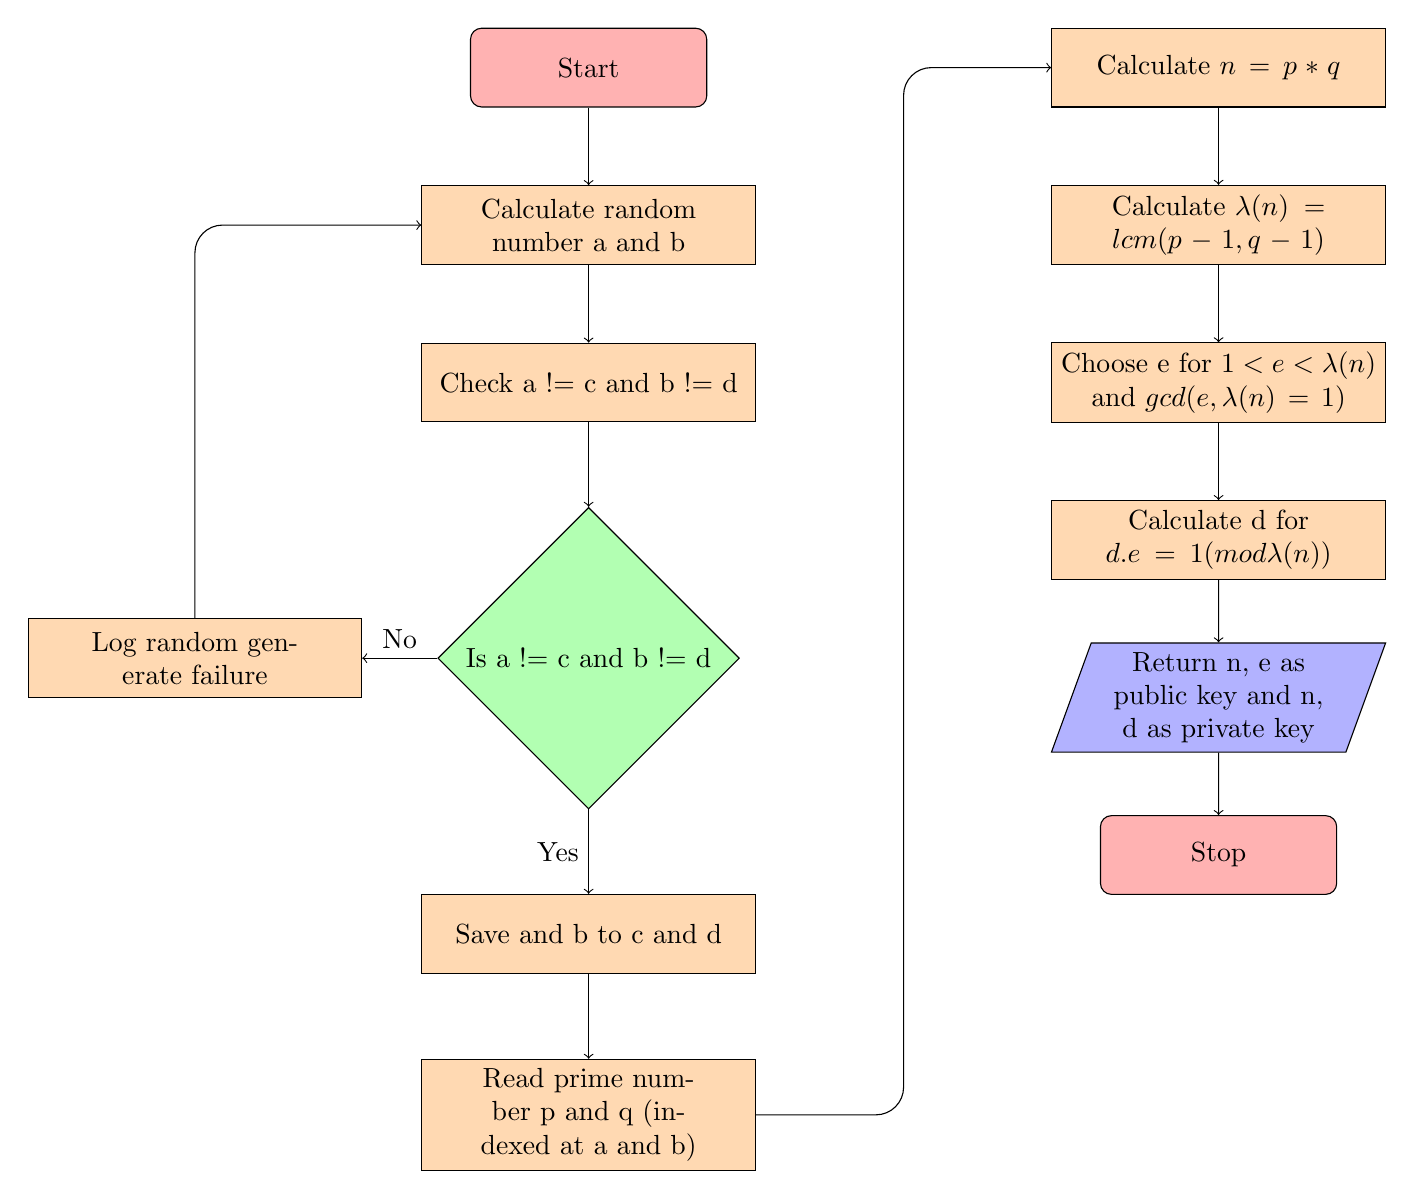
\begin{tikzpicture}[node distance=2cm, baseline = -5ex]	
    \node [startstop]												(start)			{Start};
    \node [process, below of=start]									(rand)			{Calculate random number a and b};
    \node [process,below of=rand]									(check)			{Check a != c and b != d};
    \node [decision, below of=check, yshift=-1.5cm]					(checkresult)	{Is a != c and b != d};
    \node [process, below of=checkresult, yshift=-1.5cm]			(storeab)		{Save and b to c and d};
    \node [process, below of=storeab, yshift=-0.3cm]				(prime)			{Read prime number p and q (indexed at a and b)};
    \node [process, left of = checkresult, xshift=-3cm]				(rgfail)		{Log random generate failure};
    \node [process, right of=start, xshift=6cm]						(ncalc)			{Calculate $n = p*q$};
    \node [process, below of=ncalc]									(lamdan)		{Calculate $\lambda(n) = lcm(p-1,q-1)$};
    \node [process, below of=lamdan]								(selecte)		{Choose e for $1<e<\lambda(n) $ and $gcd(e,\lambda(n)=1)$};
    \node [process, below of = selecte]								(cald)			{Calculate d for $d.e=1 (mod \lambda(n))$};
    \node [io, below of=cald]										(result)		{Return n, e as public key and n, d as private key};
    \node [startstop, below of=result]								(finish)		{Stop};
    
    \draw [->] (start) -- (rand);
    \draw [->] (rand) -- (check);
    \draw [->] (checkresult) -- node[anchor=south]{No} (rgfail);
    \draw [->, rounded corners=10pt] (rgfail) |- (rand);
    \draw [->] (check) -- (checkresult);
    \draw [->] (checkresult) -- node[anchor=east]{Yes} (storeab);
    \draw [->] (storeab) -- (prime);
    \draw [->, rounded corners=10pt] (prime) -| (4,0) -- (ncalc);
    \draw [->] (ncalc) -- (lamdan);
    \draw [->] (lamdan) -- (selecte);
    \draw [->] (selecte) -- (cald);
    \draw [->] (cald) -- (result);
    \draw [->] (result) -- (finish);
    \end{tikzpicture}
    \caption{Key generation}
    \label{fig:my_label}
\end{figure}



\newpage
\subsubsection{Modular Exponentiation}
To compute modular exponentiation of a number ($num^e\hfill mod \hfill m$), we use BigMod recursive algorithm.
\begin{figure}[H]
	\centering
	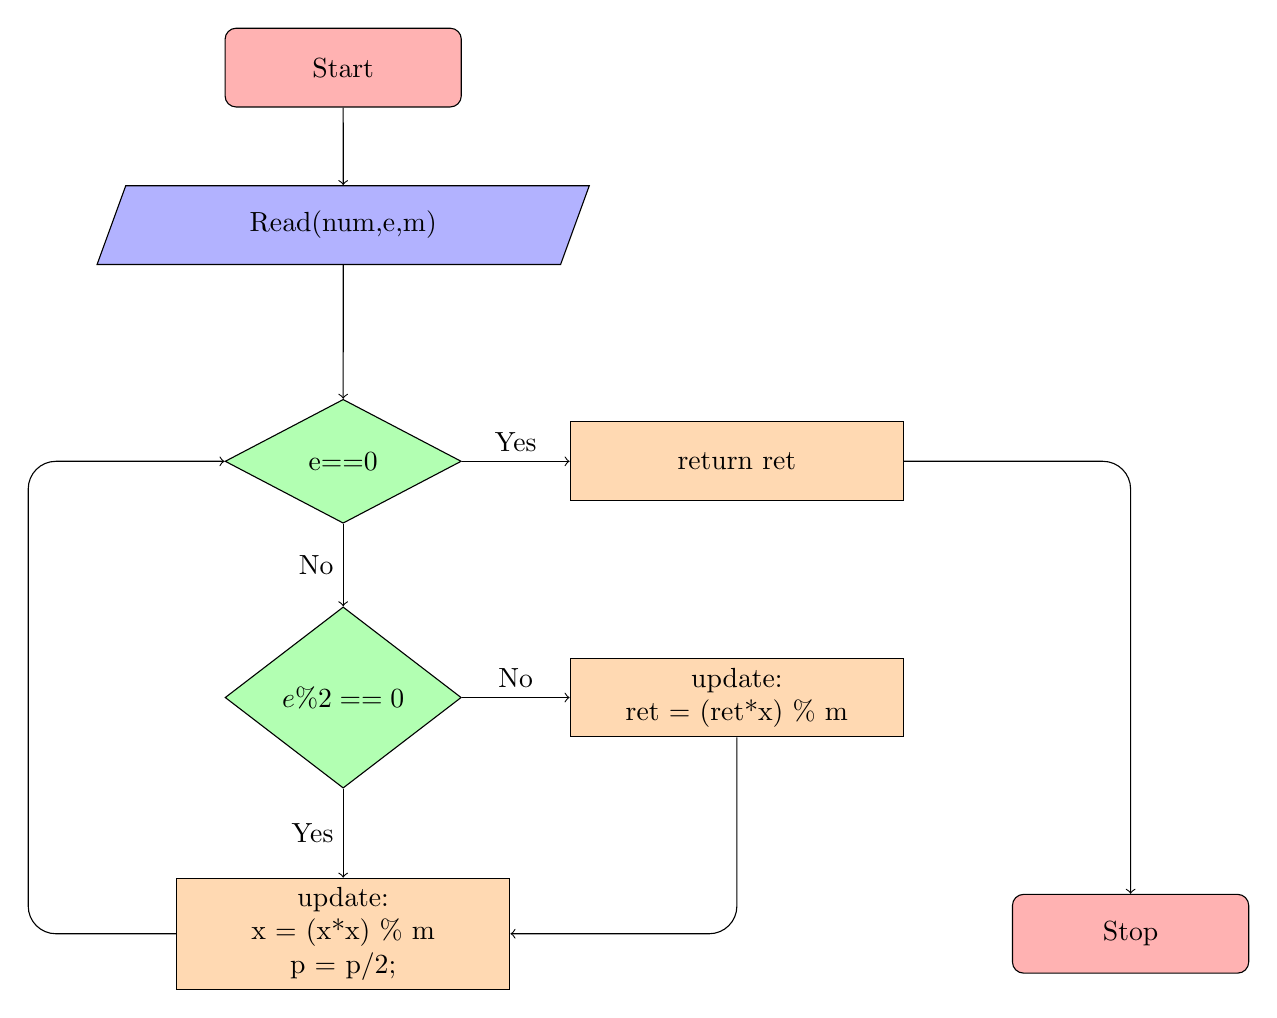
\begin{tikzpicture}[node distance=2cm, baseline = -5ex]
		\node [startstop] (init) {Start};
		\node [io, below of=init, node distance=2cm] 				(read) 		{Read(num,e,m)};
		\node [decision, below of=read, node distance=3cm] 			(decide0)	{e==0};
		\node [process, right of=decide0,node distance=5cm] 		(return1)	{return ret};
		\node [decision, below of=decide0, node distance=3cm] 		(decide1) 	{$e\%2==0$};
		\node [process, right of=decide1, node distance=5cm]    	(call1)		{update:\vfill ret = (ret*x) \% m};
		\node [process, below of=decide1, node distance=3cm]		(call2)		{ update: \vfill x = (x*x) \% m \vfill p = p/2; };	
		\node [startstop, right of=call2, xshift=8cm] (stop) {Stop};
		
		\draw [->] (init)-- (read);
		\draw [->] (read) --(decide0);
		\draw [->] (decide0)--node[above,sloped]{Yes}	(return1);
		\draw [->] (decide0)--node[left]{No} 			(decide1);
		\draw [->] (decide1)--node[above]{No} 			(call1);
		\draw [->] (decide1)--node[left]{Yes} 			(call2);
		\draw [->,rounded corners=10pt] (call1)|-(4,-11)--(call2);
		\draw [->,rounded corners=10pt]	(call2)-|(-4,-5)--(decide0);
		\draw [->,rounded corners=10pt] (return1) -| (stop);
	\end{tikzpicture}
	\caption{Modular Exponentiation}
\end{figure}


\end{document}
